% !TEX root = ./../../_Thesis.tex

% chapter's came and label
\chapter{Conclusion}
\label{chap:Discussion}

This thesis described a technique for simulating the visual perception of monochromatic images observed by an optical systems with aberrations. It assumes that all elements of a given target image are at the same known distance from the observer. 
%The technique is based on Fourier optics. 
We have validated the results of our simulations against images captured by a DSLR camera with the addition of external lenses to induce the simulated aberrations. 
% simulate myopia, hyperopia, and astigmatism.
%to simulate and validate how such aberrations affect vision.
Although this solution is able to take into account high-order aberrations, our focus was on not relying on the availability of expensive equipments, such as Shack-Hartmann wavefront sensors. 
For this, we have focused on simulating low-order aberrations (\ie, myopia, hyperopia, and astigmatism), which can be done directly from the data available on one's eyeglasses prescription.  
% (\ie, myopia, hyperopia and astigmatism) of ones optical systems and validating the results with an optical ground truth.

We have demonstrate the effectiveness of our technique by comparing the results of forty simulations against optical ground truths captured by a camera. For this, we have used three objective metrics: SSIM, PSNR, and the absolute differences of the images. 
%Histograms of two of these metrics are presented in Figure~\ref{fig:hists}. 
For all results the SSIM values are between 0.91 and 0.987 (mean = 0.93 and standard deviation = 0.02), indicating that our simulations indeed produce results that are structurally very similar the ground truths. Regarding the PSNR metric, the values vary from 29.50 to 39.37 (mean = 35.50 and standard deviation = 2.14). Such PSNR values, given in decibels, indicate that the simulation outcomes are indistinguishable from the optical ground truth captured by a DSLR camera. The absolute differences of the images reinforces the findings of the SSIM and PSNR metrics.

This thesis also described an attempt to estimate the spherical equivalent refraction of a person based on the detection of his/her absolute threshold for vision. For this, we have designed a series of experiments and a device. While the hypothesis that supports the technique sounds plausible, a reliable determination of one's absolute threshold is not a trivial task. It seems to depend on the use of high doses of cycloplegic eyedrops, making the strategy unattractive for practical use. 
%The absolute threshold psychophysical experiment allowed us to assess its use in order to estimate the spherical equivalent error of an optical system. However, due to its variability and the high number of eye drops necessary to guarantee no crystalline lens' accommodation, we could not find such relation.

%Our approach uses Fourier tools and a camera to simulate and validate results of how low-order aberrations affect vision. Even though that results seems to be visually correct, we've adopted two objective metrics to compare our results with the optical ground truth. In addition, this thesis has demonstrated the results of psychophysical studies of the absolute threshold. However, due to the crystalline lens involuntary accommodation, this intrinsic characteristic cannot be used to estimate the spherical equivalent refraction.

%Although our solution is be able to take into account the individual's refractive high-order aberrations, our focus is on not relying on the availability of expensive equipment, such as Shack-Hartmann wavefront sensors. For this, we estimate the low-order-aberration components of the individual's PSFs directly from his/her eyeglasses or contact lenses prescriptions, and use them to simulate the perception of Sloan letters. Given its reduced input need, our technique can help doctors, patients, and teachers to experiment the visual complaints.

%\begin{figure}[!b]
	%\centering
	%
	%\subfigure[]{
		%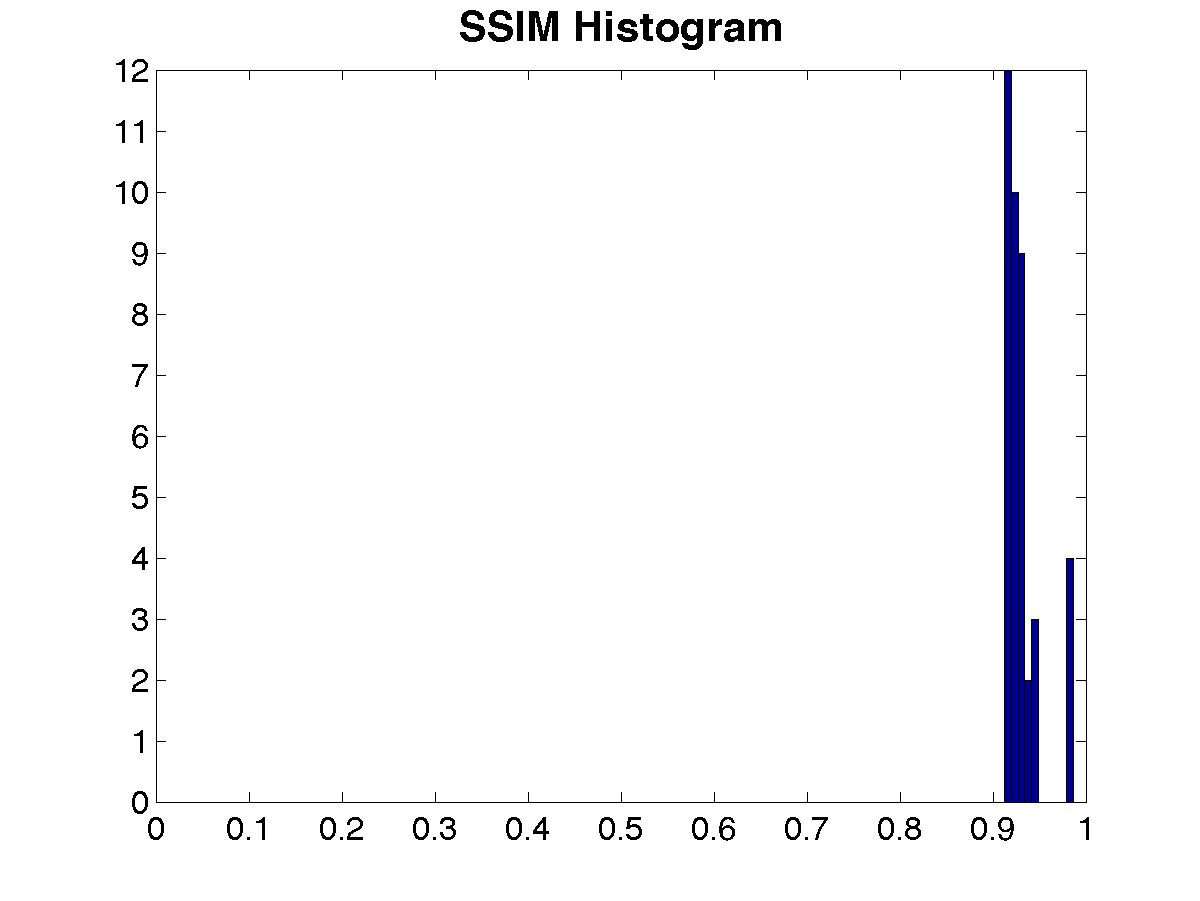
\includegraphics[width=0.47\linewidth]{__Images/05/hist-ssim.png}
		%\label{fig:hist_ssim}
	%}
	%~
	%\subfigure[]{
		%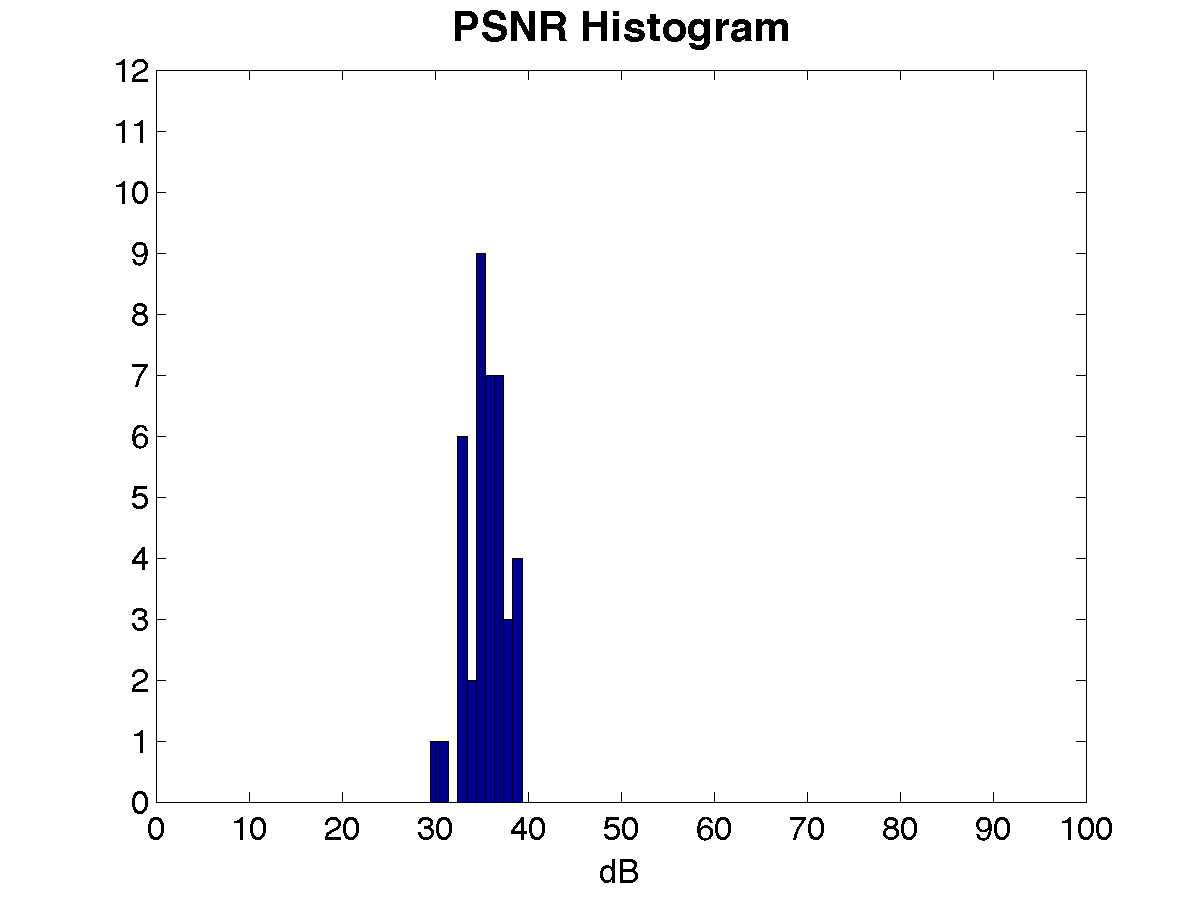
\includegraphics[width=0.47\linewidth]{__Images/05/hist-psnr.png}
		%\label{fig:hist_psnr}
	%}
		%
	%\caption[Histogram of SSIM and PSNR]{Histogram of SSIM (a) and PSNR (b) }
	%\label{fig:hists}
%\end{figure}


% Conclusions and Future Work Section
% !TEX root = ./../../_Thesis.tex

% section's Name and Label
\section{Future Work}
\label{sec:ConclusionsFutureWork}

Because visual blurring is a depth-dependent phenomenon, we would like to capture image and depth information from the environment and generate real-time simulations of how low-order aberrations affect visual  perception. Also, 
%we suppose that, by assuming 
we would like to include information about the absolute threshold in the simulation to improve its result. 
%In a way that, for example, we could generate images or design displays focusing on intrinsic perception, which cannot be corrected with ordinary eyeglasses.

%It would be interesting to study the best objective metric to compare results. Also, 
For a qualitative validation, it would be desirable to simulate the visual perception of a number of individuals who use eyeglasses. We could then ask these subjects to compare several scenes observed without their eyeglasses with the corresponding simulated views, this time with their eyeglasses on. Such an experiment could indicate how well the simulation approximates their actual vision.

% XYZ Section
% \input{__Text/06_Discussion/620.tex}

% XYZ Section
% \input{__Text/06_Discussion/630.tex}

% XYZ Section
% \input{__Text/06_Discussion/640.tex}

% XYZ Section
% \input{__Text/06_Discussion/650.tex}